% Using KOMA Script document style
% Font size setting and
% option to skip empty lines as new paragraphs
\documentclass[10pt,a4paper]{article}
% Packages without Options
\usepackage{
	algorithm,
	alltt,
	algpseudocode,
	amsfonts,
	amssymb,
	appendix,
	array,
	booktabs,
	dirtree,
	enumitem,
	float,
	footnote,
	gensymb,
	geometry,
	graphicx,
	interval,
	karnaugh-map,
	lipsum,
	listings,
	longtable,
	makecell,
	mathtools,
	minted,
  nicematrix,
	parskip,
	pdfpages,
	pgfkeys,
	pgfplots,
	subcaption,
	tabularx,
	tablefootnote,
	textcomp,
	tikz,
    titlecaps,
	venndiagram,
	wrapfig,
	wrapfig,
	xcolor
}



% Packages with Options

\usepackage[framemethod=tikz]{mdframed}
\usepackage[colorlinks,linkcolor=cyan, citecolor=cyan, urlcolor=cyan]{hyperref}
\usepackage[labelfont=bf,textfont=it,labelsep=period]{caption}
\usepackage[RPvoltages]{circuitikz}
\usepackage[english]{babel}
\usepackage[nameinlink,noabbrev]{cleveref}

\definecolor{mintedbackground}{rgb}{0.97,0.97,0.97}

\setminted[cpp]{
bgcolor=mintedbackground,
    linenos=true,
    breaklines=true,}

\setminted[js]{
bgcolor=mintedbackground,
    linenos=true,
    breaklines=true,}

\setminted[python]{
bgcolor=mintedbackground,
    linenos=true,
    breaklines=true,}
    

\linespread{1.5}

% Package: AlgorithmicX
% Sets all comments to be indentend and aligned

\renewcommand{\Comment}[2][.7\linewidth]{%
  \leavevmode\hfill\makebox[#1][l]{//~#2}}


% Package: Interval
% Sets the style of mathematical intervals
\intervalconfig{
soft open fences, separator symbol=,,
}

% Package: Geometry
% Sets the page margins
\geometry{
    a4paper,
    left=32mm,
    right=22mm,
    top=22mm,
    }
	
% Creates a proper caption name for algorithms
\newcommand{\algorithmautorefname}{Algorithm}
\newcommand{\listingautorefname}{Listing}
\algrenewcommand{\algorithmiccomment}[1]{\texttt{// #1} }
% Creates a numbered environment for Theorems
\newtheorem{theorem}{Theorem}

% Redefine the implication arrow to be a simple, thin arrow instead of the default, thick arrow
\renewcommand{\implies}{\rightarrow}

% Create a new command for the set complement to make my logical statements easier to read
\newcommand{\compl}{\overline}

% Creates commands for combinatorics nCr and nPr
\newcommand{\nCr}[2]{\,_{#1}C_{#2}} % nCr
\newcommand{\nPr}[2]{\,_{#1}P_{#2}} % nPr

% Package: tikz
% Loads libraries for drawing automata, 
\usetikzlibrary{automata,positioning,shadows,arrows, shapes.gates.logic.US, calc}

% Creates a command to create a button shape
\newcommand*\keystroke[1]{%
  \tikz[baseline= (key.base)]
    \node[%
      draw,
      fill=white,
      drop shadow={shadow xshift=0.25ex,shadow yshift=-0.25ex,fill=black,opacity=0.75},
      rectangle,
      rounded corners=2pt,
      inner sep=1pt,
      line width=0.5pt,
      font=\scriptsize\sffamily
    ] (key) {#1\strut};
}

% Package: pgfplot
% Sets the global options for PGF Plots
\pgfplotsset{compat=newest}

% Package: tikz
% Flowchart Shapes
\tikzstyle{startstop} = [rectangle, rounded corners, minimum width=3cm, minimum height=1cm,text centered, draw=black, fill=red!30]
\tikzstyle{io} = [trapezium, trapezium left angle=70, trapezium right angle=110, minimum width=3cm, minimum height=1cm, text centered, draw=black, fill=blue!30]
\tikzstyle{process} = [rectangle, minimum width=3cm, minimum height=1cm, text centered, draw=black, fill=orange!30]
\tikzstyle{decision} = [diamond, minimum width=3cm, minimum height=1cm, text centered, draw=black, fill=green!30]
\tikzstyle{arrow} = [thick,->,>=stealth]

% Disable Minted syntax error highlights (red boxes)
\AtBeginEnvironment{minted}{%
  \renewcommand{\fcolorbox}[4][]{#4}}

% Listings Style (non-minted)

\lstdefinestyle{arjuncode}{
    basicstyle=\ttfamily,
    breakatwhitespace=false,         
    breaklines=true,                 
    captionpos=b,                    
    keepspaces=true,                 
    numbers=left,                    
    numbersep=5pt,                  
    showspaces=false,                
    showstringspaces=false,
    showtabs=false,                  
    tabsize=2
}

\lstset{style=arjuncode}

\graphicspath{{images/}}

 %Adjust this based on where your Summary is stored
\title{CM3020: Artificial Intelligence \\ Summary}
\author{Arjun Muralidharan}
\begin{document}

\maketitle
\newpage
\tableofcontents
\listoffigures
\listoftables
% \listofalgorithms

\newpage
\renewcommand{\subsubsectionautorefname}{section\negthinspace}

\section{Evolving creatures with genetic algorithms}
\begin{mdframed}
    \textbf{Learning Outcomes}
    \begin{itemize}[label={\checkmark}]
        \item Describe and discuss key issues in a range of branches of Artificial Intelligence.
        \item Select appropriate artificial intelligence algorithms for particular scenarios and evaluate their adequacy and efficiency using appropriate techniques
        \item Create working computer programs that implement specific artificial intelligence techniques
        \item Describe how information can be represented in an artificial intelligence system and select appropriate representations for different types of information
    \end{itemize}
\end{mdframed}

\subsection{Introduction to evolution theory}

\subsubsection{Bio-Inspired Computing}

\textbf{Bio-inspired computation} has emerged as one of the most studied branches of AI during the last decades.

\paragraph{Cybernetics (1950s)} The science of control and communication in the animal and the machine. Co-ordination, regulation and control will be its themes, for these are of the greatest biological and practical interest.

\paragraph{Connectionism (1960s)} The perceptron is a minimally constrained ``nerve net'' consisting of logically simplified neural elements, which has been shown to be capable of learning to discriminate and to recognize perceptual patterns. \textit{This is the birth of deep neural networks.}

\paragraph{Artificial Life (1980s)} Simulation of evolution, bio-primordial chemistry, completely artificial complex systems and more. \textit{``Life as it could be''}.

\paragraph{Genetic Algorithms} Procedures that allow you to solve problems with iterative solutions.

\subsubsection{Evolution Theory}

Darwin proposed three generalisations:

\begin{enumerate}
    \item Variation: no two individuals are identical within a population.
    \item Hereditary characteristics: the variation expressed as individual characteristics is in heritable from parents to offspring.
    \item Multiplication and competition: Malthus’s observation --- about population increase where no competition for resources exists —-- means that as resources are always finite, competition must act as a brake on population growth.
\end{enumerate}

If these forces act, then hereditary variations within a population that allowed an organism to survive were more likely to be passed down. This process is called natural selection.

A \textbf{genotype} encodes the characteristics of the individual. This is expressed in DNA as the strands of the double-helix. A \textbf{phenotype} is the actual individual that manifests in the world. It is the actual expression of the genotype when taking environmental factors into consideration.

\textbf{DNA} is made up of four nucelobases, \textit{adenine (A)}, \textit{guanine (G)}, \textit{cytosine (C)}, and \textit{thymine (T)}. DNA gets converted into proteins that then define how an individual works. These combine with sugars and phosphates to create \textit{nucelotides}, which are the molecules making up DNA.

The nucelotides of an individual then gets mapped to 21 different amino acids, which then form proteins. In 2021, DeepMind was able to model and predict which amino acids get expressed as what proteins (\href{https://deepmind.com/research/open-source/alphafold-protein-structure-database}{AlphaFold}).

The environment applies \textbf{selective pressure} to phenotypes. \textbf{Fit} phenotypes are more likely to reproduce.

\textbf{Fitness landscapes} describe the peaks and thoughs of evoluationary success within a population.

\begin{itemize}
    \item An individual within a species is represented as a string of genes that defines its genotype. The string itself has a real number associated with it.
    \item This number defines the fitness of the string in terms of the phenotype it produces.
    \item The distribution of fitness values over the space of all genotypes gives the fitness landscape, and all members of the population map onto that landscape according to their fitness value.
    \item Selection and mutation causes individuals to ``walk'' to the nearest peak.
\end{itemize}

Simple fitness landscapes only map two traits in relation to each other and can be visualised in a 3D surface graph (with the height being the level of fitness).

\begin{figure}[ht]
    \centering
    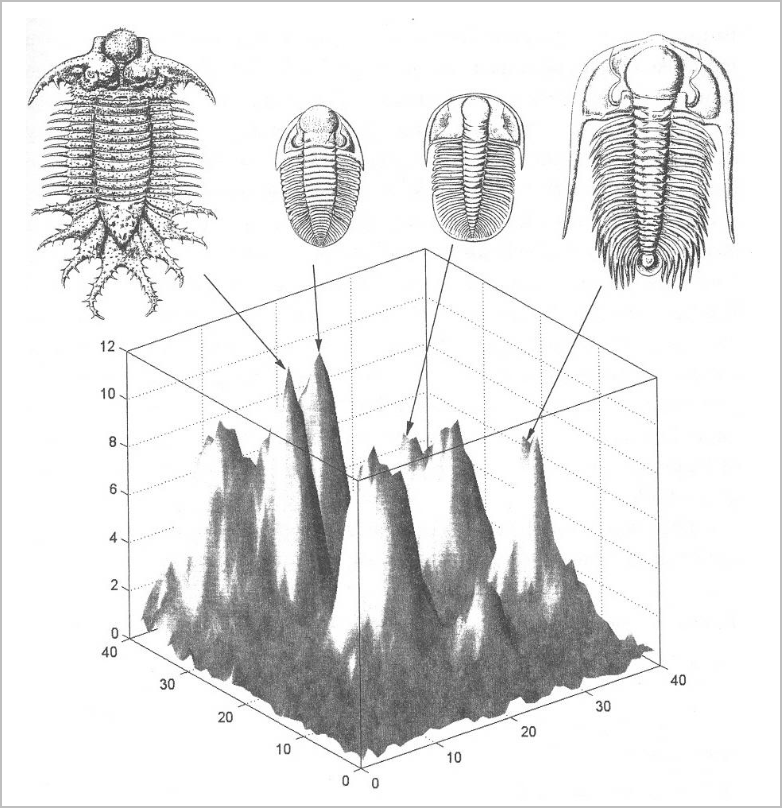
\includegraphics[width=8cm]{fitnesslandscape.png}
    \caption{Fitness Landscapes}
    \label{fig:fitness}
\end{figure}

\subsection{Artificial Evolution and Genetic Algorithms}

\textbf{Genetic algorithms} are \textit{probabilistic search procedures} designed to work on large spaces involving \textit{states} that can be represented by \textit{strings}.

With regards to evolution theory, probabilistic search represents \textit{selection}, while the states relate to \textit{phenotypes} and the strings are the \textit{genotypes}.

The \textit{search space} is a space of possible solutions to a problem. If we can search the space, we can find a solution.

The space can be represented by the length for a \textit{bit string}, with the possible values being the genotypes, and an actual value for the bit string would be the phenotype.

Each phenotype that is found in the space is given a \textbf{fitness score}. The fitness score is then used to determine the likelihood of this individual being selected for breeding.

An analogy is to map the fitness scores to the angles of a \textbf{roulette wheel}, spinning the wheel and selecting two parents. The fittest invidiuals are more likely to get selected, but it is still possible for others to get selected.

Breeding consists of two steps: \textbf{Mutation} and \textbf{Crossover}.

\paragraph{Crossover} Takes parts of one parent's genome and the other part from the other parent. A basic version is \textit{single point crossover} where the entire sequence up to a digit is taken from parent A, and the rest from parent B. This could be selected at random.

\paragraph{Mutation} Once the crossover is done, the new genotype gets some bits flipped randomly, which represents a mutation. This is then expressed in a new phenotype with crossover and mutation elements.


Based on this theory, a canonical form of a \textbf{genetic algorithm (GA)} was formulated:

\begin{enumerate}
    \item Set $t = 0$
    \item Initialise chromosome population $P(t)$.
    \item Evaluate $P(t)$ using fitness criteria
    \item \textbf{while} termination condition not satisfied \textbf{do}
    \item \begin{enumerate}
              \item Select best individuals from $P(t)$. Let P1(t) be the set of selected chromosomes. Choose individuals from $P_{1}(t)$ to enter mating pool $(MP)$.
              \item Recombine chromosomes in MP forming populations $P_2$. Mutate chro- mosomes in $P_2$ forming $P_3$.
              \item Select replacements from $P_3$ and P (t) forming $P (t + 1)$.
              \item Set $t=t+1$
          \end{enumerate}
\end{enumerate}

\subsubsection{Why do genetic algorithms work?}

Genetic algorithms try to find a \textbf{global maximum} of the fitness function in a multi-dimensional space.

\textbf{Hyperplane sampling} is a technique that breaks down a problem into components that can be recombined over and over so we can test different solutions.

\textbf{Schema theorem} says that there are patterns (schemas) like a simple regular expression. For example, we could freeze some bits of the genotype and iterate other bits by defining a schema to use (e.g. 100****1 would use the fixed bits but try out different bits for the *).

\paragraph{Implicit parallelism} takes the population and compares two individuals in sequence, one at a time.

\paragraph{Computational parallelism} applies this to a computing environment, where you can evaluate multiple pairings individuals in parallel computing threads, depending on how many cores your processor has.

\subsubsection{Karl Sims Creatures}

\paragraph{Evolving Morphology} \textit{Dawkin's Biomorphs} express the idea that evolution can create very complicated morphologies over time through the process of iteration. Using small mutations of biomorphs - abstract figures made to look vaguely like creatures in nature, Dawkins clearly showed how the process of evolution can create very complicated organisms if given a long period of time.

It is presented as a counter-argument to the idea of `intelligent design` - where the complexity of life is said to attest to the existence of a higher creator-being, commonly denoted as `God`.

\paragraph{Sims Creatures} Karl Sims' paper from 1994 describes a system for creating virtual creatures that move and behave in sumulated 3D physical worlds.

\paragraph{Creature morphology} The morphology or genotype is represented as a \textbf{directed graph} where the nodes are similar to joints and the vertices are the movable ``arms'' of the creature.

The graph can contain \textit{multiple connections}, meaning that a node with multiple connections to another node means that the directed node is repeated multiple times.

The graph can also contain \textit{recursion}, so an edge from a node to itself means that the node is connected to another identical node.

\paragraph{Creature neural architecture} Mapping from sensor input to actuator output. The graph as a whole percepts some input and produces an output for that input.


\section{Intelligent Agents}

\textit{Summary of Chapter 2 from Russell/Norvig}

In AI, we generally want to build \textit{rational agents}. Rationalaity is defined as acting in a way that achieves the best expected outcome.

An agent is anything that \textit{perceives} its \textit{environment} through \textit{sensots} and takes action upon the environment through \textit{actuators}.

The \textbf{percept sequence} is a history of all percepts of an agent, and the \textbf{agent function} maps any given percept sequence to an action.

\paragraph{Definition of a rational agent} For each possible percept sequence, a rational agent should select an action that is expected to maximize its performance measure, given the evidence provided by the percept sequence and whatever built-in knowlege the agent has.

\textit{Note: Rationality does not mean omniscience, rather, rationality deals with expected performance, not absolute certainty.}

A \textbf{task environment} is defined as consisting of:

\begin{itemize}
    \item \textbf{Performance Measure:} The desired outcome of our agent.
    \item \textbf{Environment:} The full, partially or un-observable environment of the agent.
    \item \textbf{Actuators:} The means by which the agent can act on the environment.
    \item \textbf{Sensors:} The means by which the agent can perceive the environment, and store a percept sequence.
\end{itemize}

\subsection{Properties of Task Environments}

\paragraph{Fully observable vs. partially observable} How much of the environment can a single percept through sensors perceive?

\paragraph{Single-agent vs. multi-agent} How many agents are acting, and are they \textbf{competitive} or \textbf{cooperative} (or neither).

\paragraph{Deterministic vs. non-deterministic} Is the next state of the environment completely determined by the action of the agent? If non-deterministic, is the probability of outcomes known (is it \textit{stochastic})?

\paragraph{Episodic vs. Sequential} Do actions impact future actions?

\paragraph{Static vs. Dynamic} Does the environment change while the agent is deciding on the action?

\paragraph{Discrete vs. continuous} Does the agent need to act on discrete environments (e.g. single objects) or a continuous environment through the flow of time?

\paragraph{Known vs. unknown} How much has the designer of the agent built-in knowledge about the world?


\subsection{Agent Programs}

A basic agent program is defined as taking a \textit{percept}, appending this to the \textit{percept history}, looking up an action in a table representing the agent function, and returning the action. The percept history and table are persistent elements of such an agent, and would be programmed as persistent data of an object.

\paragraph{Simple Reflex Agents} These agents select an action based solely on the \textit{current} percept and refer to a set of \textit{condition-action rules} to decide the action. A common problem is running into infinite loops (because the agent doesn't use previous percepts and might try the same thing over and over again), which can be overcome by \textbf{randomization} of actions (e.g. randomly turn left or right as a vacuum).

\paragraph{Model-based reflex agents} These agents maintain an \textit{internal state} of the environment to overcome partial observability, by storing a \textit{transition model}, which describes how the actions of the agent impact the environment and how the environment evolves independently, and a \textit{sensor model}, which describes how the current state is reflected in sensors. This agent updates its internal state using the current percept, the current state, the most recent action and the two models. It then checks the state against a set of rules and chooses the action.


\subsection{Pybullet \& URDF}

Pybullet is a physics engine that can simulate objects in a 3D environment using Python. We also use a file format called the \textbf{unified robot description format} (URDF) to describea ``creature'' in the simulation, a phenotype or specific expression in our evolutionary space.

In creating 3D simulations, it is useful to have \textbf{separate collission and visual geometry}, meaning that complex shapes are simplified when calculating collisions (e.g. a creature is surrounded by an invisible box, and the box is used for detecting collisions). This is done to manage how complex the computations will be, as more complex shapes need more computation to detect ongoing collissions.

\paragraph{URDF} An XML-based filed format for specifying robot models, including their motors and other dynamics. It's useful for programmatically generating models, and easily share models. Pybullet provides some premade models via a \texttt{data} module.

URDF files define \textbf{links} (which are the nodes) and \textbf{joints} which are the edges between the nodes. This expresses a robot as a \textbf{directed graph}.

\begin{listing}
    \label{lis:URDF}
    \caption{Basic URDF File}
    \begin{lstlisting}[language=xml]
    <?xml version="1.0"?>
        <robot name="myfirst">
            <link name="base_link">
                <visual>
                    <geometry>
                        <cylinder length="0.6" radius="0.2"/>
                    </geometry>
                </visual>
            </link>
        </robot>\end{lstlisting}\end{listing}

Note that in URDF, you need to specify the \textbf{visual} representation separately from the \textbf{collision} representation. If the latter is unspecified, objects will just never collide.


\section{Robot Scientist}

\subsection{Discovery Science}

Technology drivers for AI:
\begin{enumerate}
	\item Improved hardware
	\item Improved data availability
	\item Improved computer software
\end{enumerate}

AI has seen cycles of hype and disillusionment. This time is different, because it's at the core of large companies like GAFA.

\subsubsection{Scientific Discovery}

\begin{enumerate}
	\item Scientific Discovery
	\item Scientific problems are abstract, but involve the real-world.
	\item Scientific problems are restricted in scope no need to know about "Cabbages and Kings".
	\item Nature is honest no malicious agents.
	\item Nature is a worthy object of our study.
	\item The generation of scientific knowledge is a public good.
\end{enumerate}

\subsubsection{Legal and ethical issues in robotic science}

\paragraph{Roboethics} The study of ethical issues related to robot design, operation and use. Focus on:

\begin{enumerate}
	\item Designing robots ethically
	\item Treating robots, and robots treating people
	\item Robot rights
	\item Responsibility if robots cause harm
	\item Risks of emotional bonds with robots
	\item Ethical codes
\end{enumerate}

General issue: Robots replacing humans. AI systems can process large volumes of data, reasoning and parallel tasking.

\begin{enumerate}
	\item AI systems are better in: processing large volumes of data, reasoning and parallel tasking
	\item AI systems work 24/7
	\item humans are better in: high-level planning, making
	decisions in uncertain non-deterministic and
	partially observable environments
	\item Target: human-robot collaboration and co-creation
	\item AI systems have baises
\end{enumerate}

\subsection{Rational agents}
An \textbf{agent}  is a system that perceives its environment through its sensors and acting upon that environment through actuators.

The \textbf{percept sequence} is the complete history of everything the agent has ever perceived.

The agent's behaviour is described by the \textbf{agent function} that maps any given percept sequence to an action. You could tabulate all percept sequences and the resulting actions, which would be infinite unless percept sequences are bounded. If agents act \textit{randomly}, then the tabulation for the same percept sequence would need to be done many times to capture the probability of each action happening.

\paragraph{Example: Vacuum cleaners} Assuming a vacuum cleaner with only two locations to clean, the perecept sequence might consist of the current location and the dirtyness of the current location. If the current location is clean, move to the other location. If it is dirty, start cleaning here. This evaluation of reality is repeated.

A \textbf{rational agent} is one that does the right thing. We evaluate it's behaviour cased on it's \textbf{consequences}.

\paragraph{Rationality} For each possible percept sequence, a rational agent should select an action that is expected to maximize it's performance measure, given the evidence provided by the percept sequence and whatever built-in knowledge the agent has.

\subsubsection{Environments}

An agent operates in a \textbf{task environment} described by the \textbf{performance} measure, \textbf{environment}, \textbf{actuators} and \textbf{sensors} involved in performing a task.

Task environments can be classified in the following dimensions:

\begin{enumerate}
	\item \textbf{Fully observable vs. partially observable}: Do the sensors have access to the complete state of the environment? 
	\item \textbf{Single-agent vs. multi-agent}: If multiple agents are involved, are they \textbf{competitive} or \textbf{cooperative}?   
	\item \textbf{Deterministic vs. non-deterministic}: Is the next state of the environment completely determined by the current state and action executed?
	\item \textbf{Episodic vs. sequential}: Do the actions taken depend on actions taken in previous "episodes"? Does the current action influence future actions? For example, detecting faulty parts in an assembly line is episodic, driving a car is sequential. 
	\item \textbf{Static vs. dynamic}: Can the environment change while the agent is deliberating an action?
	\item \textbf{Discrete vs. continuous}: Are the set of percepts and actions discrete (game of chess) or continuous (driving a car)?
	\item \textbf{Known vs. unknown} Does the agent have a knowledge representation about the environment? 
\end{enumerate}

The hardest case is partially observable, multi-agent, nondeterministic, sequential, dynamic, continuous and unknown.













A meta-analysis agent collects information about runs, results, and compares performance of other agents

A collaboration agent supports a team of robot scientists or a team of human and robot scientists

A monitoring agent monitors and records everything what is happening 

An external services agent is an interface for external users

A model agent works with executable computational models and runs simulations

An explanation agent produces explanations about the working of the system and its conclusions


\end{document}

